\documentclass[10pt,conference]{IEEEtran}
% The preceding line is only needed to identify funding in the first footnote. If that is unneeded, please comment it out.
\usepackage{cite}
\usepackage{amsmath,amssymb,amsfonts}
\usepackage{algorithmic}
\usepackage{graphicx}
\usepackage{textcomp}
\usepackage{xcolor}
\usepackage{fancyhdr}
\usepackage[outputdir=docs]{minted}
\usepackage{amsthm}

\def\abstractname{Abstrak}
\def\IEEEkeywordsname{Kata Kunci}
\def\refname{Daftar Pustaka}

\theoremstyle{definition}
\newtheorem{definition}{Definisi}[section]

\newtheorem{theorem}{Teorema}[section]

\def\BibTeX{{\rm B\kern-.05em{\sc i\kern-.025em b}\kern-.08em
    T\kern-.1667em\lower.7ex\hbox{E}\kern-.125emX}}

\graphicspath{{./src/img}}

%%% Footer Left
\makeatletter

\def\ps@headings{
\let\@oddhead\@empty
\let\@evenhead\@empty
\def\@oddfoot{Makalah IF2120 Matematika Diskrit – Sem. I Tahun 2021/2022\hfill}
\def\@evenfoot{Makalah IF2120 Matematika Diskrit – Sem. I Tahun 2021/2022\hfill}
}

\def\ps@IEEEtitlepagestyle{% default title page headers, no footers
\let\@oddhead\@empty
\let\@evenhead\@empty
\def\@oddfoot{Makalah IF2120 Matematika Diskrit – Sem. I Tahun 2021/2022\hfill}%
\let\@evenfoot\@empty
}
\makeatother

\pagestyle{headings}

% Document

\begin{document}

\title{Penerapan Pembangkit Bilangan Acak dalam Steganografi}

\author{\IEEEauthorblockN{Bayu Samudra - 13520128\textsuperscript{1}}
\IEEEauthorblockA{\textit{Program Studi Teknik Informatika} \\
\textit{Sekolah Teknik Elektro dan Informatika}\\
Institut Teknologi Bandung, Jl. Ganesha 10 Bandung 40132, Indonesia \\
\textsuperscript{1}13520128@std.stei.itb.ac.id}
}

\maketitle

\begin{abstract}
Testing This document is a model and instructions for \LaTeX.
This and the IEEEtran.cls file define the components of your paper [title, text, heads, etc.]. *CRITICAL: Do Not Use Symbols, Special Characters, Footnotes, 
or Math in Paper Title or Abstract.
\end{abstract}

\begin{IEEEkeywords}
Keamanan, Steganografi, \emph{Linear Congruetial Generator} (LCG)
\end{IEEEkeywords}

\section{Pendahuluan}
Dunia saat ini telah memasuki era yang penuh dengan data. Data setiap waktunya bertumbuh secara ekponensial. 
Data merupakan hal yang sangat penting bagi setiap orang. Data yang tersebar pada internet banyak jenisnya. 
Ada data yang merupakan data yang memang dibagikan untuk publik bahkan ada juga sata rahasia yang bersifat privat. 
Data yang bersifat privat ini haruslah dijaga kerahasiaannya. Sealh satu cara untuk menjaganya adalah dengan menggunakan kriptografi.

Kriptografi adalah ilmu yang mempelajari mengenai cara-cara untuk menjaga integritas dan keamanan dari suatu data.\cite{b1}
Dalam menjaga data, kriptografi menggunakan cabang-cabang ilmu matematika terutama dalam teori bilangan. 
Kriptografi juga merupakan sebuah seni. Hal ini dikarenakan pada awal kemunculannya, setiap orang memiliki 
caranya tersendiri untuk mengamankan pesannya. Terdapat banyak kriptografi klasik seperti Caesar Cipher, 
Vigenere Cipher, Affine Cipher, dan lainnya.

Selain menggunakan kriptografi, terdapat sebuah teknik lain untuk mengamankan sebuah data. Teknik ini dikenal steganografi. 
Steganografi adalah sebuah ilmu yang mempelajari teknik-teknik bagaimana menyembunyikan sebuah data dalam sebuah media sehingga 
sulit untuk dikenali. \cite{b1} Steganografi ini sudah dikenal cukup lama sejak sejak bangsa Yunani. Steganografi yang pernah 
tercatat pada zaman itu adalah saat penguasa bernama Histaiaeus, seorang penguasa Yunani, mengirimkan pesan tersembunyi kepada 
Aristagoras untuk melawan Persia. Sang penguasa mengirimkan pesan tersebut dengan membotaki para budah dan rambutnya dibiarkan tumbuh, 
lalu dikirimkanlah kepada Aristagoras. Hal ini dapat dilihat pada buku yang telah ditulis oleh Herodatus, \emph{Histories of Herodatus}.

Steganografi ini berbeda dengan Kriptografi. Pada kriptografi, data diubah menjadi sesuatu yang dapat tidak memiliki arti. 
Akan tetapi, data tersebut masih ada keberadaanya. Dalam Steganografi, data disembunyikan dalam sebuah medium sehingga tidak terlihat 
keberadaannya. Medium ini bisa apapun, baik itu gambar, video, file, atau bahkan teks. Data pada medium ini pada akhirnya harus bisa 
diekstraksi untuk diambil pesannya.

Steganografi ini memiliki kelebihan, yaitu data yang dikirimkan tidak menarik perhatian orang lain. Steganografi ini pun dapat 
diintegrasikan dengan Kriptografi untuk meningkatkan keamanan data yang disimpan.

\section{Teori Dasar}

\subsection{Terminologi Dasar Steganografi}

Dalam Steganografi, dikenal beberapa terminologi dasar. Berikut ini adalah beberapa terminologi dasar yang perlu diketahui: \cite{b1}

\begin{itemize}
    \item Pesan tersembunyi adalah pesan yang disisipkan pada sebuah medium baik itu berupa video, image, audio, ataupun teks. 
    \item Cover adalah media yang digunakan untuk menyisipkan pesan.
    \item \emph{Stego-object} adalah media yang telah tersisipkan pesan tersembunyi di dalamnya.
    \item Steganalisis adalah cabang ilmu yang membahas mengenai pendeteksian pesan tersembunyi yang ada pada sebuah media. Terdapat 
    beberapa jenis metode dalam steganalisis ini yang akan dijelaskan pada bagian selanjutnya.  
\end{itemize}

\subsection{Kriteria Kualitas Steganografi}
Sebuah steganografi dikatakan memiliki kualitas yang baik apabila mengikuti beberapa kriteria berikut:

\begin{itemize}
    \item \emph{Impercepibility} yaitu perubahan oleh steganografi tidak boleh dapat dirasakan oleh inderawi. Hal ini ditujukan agar
    tidak menimbulkan kecurigaan orang lain.
    \item \emph{Fidelity} yaitu perubahan oleh steganografi tidak jauh mengurangi kualitas dari suatu cover. Misalkan pada cover gambar,
    steganografi tidak boleh membuat gambar tersebut menjadi pecah.
    \item \emph{Recovery} yaitu pesan yang disisipkan oleh proses steganografi haruslah bisa diekstraksi kembali.
    \item \emph{Payload} yaitu pesan yang disisipkan dapat dimuat sebanyak mungkin.
    \item \emph{Robustness} yaitu \emph{stegeo-object} harus tahan terhasap serangan padanya. Akan tetapi, aspek in
    tidak terlalu dipentingkan karena steeganografi menyembunyikan pesan sehingga tidak menimbulkan kecurigaan.
\end{itemize}

\subsection{Jenis Steganalisis}
Steganalisis terbagi menjadi beberapa jenis. Berdasarkan kespesifikannya, steganalisis dibagi menjadi dua jenis, yaitu sebagai berikut
\begin{itemize}
    \item \emph{Targeted Steganalysis} yaitu steganalisis yang membatasi analisis pada media atau algoritma steganografi tertentu. 
    \item \emph{Blind Steganalysis} yaitu steganalisis yang menganalisis dari berbagai algoritma dan format media. Hasil statistik dar
    setiap data akan dibandingkan dan diambil kesimpulan.
\end{itemize}

Selain berdasarkan kespesifikannya, steganografi juga dibagi menjadi menjadi dua berdasarkan metode yang digunakan.
\begin{itemize}
    \item \emph{Visual Steganalysis} yaitu steganalisis yang dilakukan dengan indera visual. Steganalisis jenis ini bersifat sujektif.
    \item \emph{Statistical Steganalysis} yaitu steganalisis yang menganalisis menggunakan analisis matematika terutama menggunakan statistika.
\end{itemize}

\subsection{Representasi Bilangan Bulat}
Pada dasarnya, komputer menyimpan dan memproses informasi dalam bentuk sinyal duanilai. Setiap sinyal tersebut merepresentasikan angka 
dalam bentuk bit. Kumpulan dari berbagai bit dapat memberikan makna dari suatu data  yang sedang diproses. Kumpulan dari berbagai bit ini 
dapat membantuk sebuah bilangan yang disebut dengan bilangan biner.

Dalam dunia keinformatikaan, terdapat dua jenis representasi bilangan bulat yang sering digunakan yaitu sebagai berikut:
\begin{itemize}
    \item \textbf{Bilangan Biner} \\
    Bilangan biner yaitu bilangan dengan basis dua. Bilangan biner hanya terdapat dua simbol yang tersedia, yaitu 0 dan 1. Konversi bilangan 
    biner ke bilangan desimal didefinisikan pada persamaan 1.
    
    \begin{equation}
         d = \sum_{i=0}^{n} b_i \cdot 2^{i}
    \end{equation}

    Nilai $ b_i $ melambangkan digit biner ke-i dan $ d $ adalah bilangan desimal hasil konversi. \\


    \item \textbf{Bilangan Hexadesimal} \\
    Bilangan Hexadesimal adalah bilangan dengan basis 16. Dua digit dari bilangan ini merepresentasikan satu byte (8-bit). Bilangan Hexadesimal 
    ini dapat meringkas penulisan biner dan juga memudahkan alam penganalisisan bilangan biner. Bilangan hexadesimal ini pada dasarnya terdiri 
    dari simbol 0 sampai dengan 9 dilanjutkan dengan simbol A,B,C,D,E, dan F. Berikut ini adalah rumus konversi bilangan heksadesimal ke bilangan desimal.

    \begin{equation}
        d = \sum_{i=0}^n h_i \cdot 16^{i}
    \end{equation}

    Nilai $ h_i $ menyatakan digit hexadesimal ke-i. Bila digit Hexadesimal bernilai $ \text{A} $ maka digantikan dengan nilai $ 10 $. Begitu 
    pula dengan nilai $ \text{B} $ yang digantikan dengan nilai 11. Hal ini berlaku seterusnya hingga $ \text{F} $.
\end{itemize}

\subsection{Signifikansi Bit}
Terdapat dua buah definisi yang perlu diperhatikan mengenai signifikansi bit.Misalkan terdapat sebuah bilangan bulat dengan $ w $-digit dan urutan 
digitnya adalah $ [b_{w-1}, b_{w-2}, \cdots, b_{2}, b_{1}, b_{0}] $. Digit $ b_{w-1} $ disebut sebagai \emph{most significant bit} atau biasa disingkat 
sebagai MSB. Bit $ b_{0} $ disebut sebagai \emph{least significant bit} atau biasa disingkat sebagai LSB.

\begin{figure}[htbp]
    \centerline{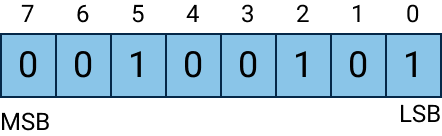
\includegraphics[width=0.9\columnwidth]{MSB-LSB.png}}
    \caption{Ilustrasi MSB dan LSB}
\end{figure}

\subsection{Citra Digital}
Pada komputer sebuah citra digital disimpan dalam kumpulan byte data. Bagian terkecil dari sebuah citra digital disebut dengan pixel. Citra digital
merupakan matriks dari pixel tersebut. Setiap pixel direpresentasikan dengan bilangan $n$-bit. Berdasarkan jumlah bit pada pixel, citra digital dapat 
diklasifikasikan menjadi beberapa jenis yaitu sebagai berikut: \cite{b1}\cite{b3}

\begin{itemize}
    \item \textbf{Citra 24-bit}\\
    Pada citra 24-bit, setiap pixel terdiri atas 3 buah kanal. Kanal pada citra ini adalah yaitu R (\emph{Red}), G (\emph{Green}), dan B (\emph{Blue}).
    Setiap kanal memiliki besar 8-bit yang merepresentasikan bilangan 0 sampai 255.

\begin{figure}[htbp]
    \centerline{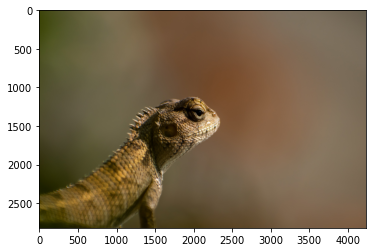
\includegraphics[width=0.9\columnwidth]{citra-original.png}}
    \caption{Citra berwarna 24-bit (Sumber: Unsplash)}
    \label{fig:24original}
\end{figure}

    \item \textbf{Citra 8-bit} \\
    Citra ini biasa disebut sebagai citra grayscale. Citra ini hanya memiliki 1 buah kanal yang menyatakan nilai keabuan. Konversi dari citra berwarna
    menjadi citra grayscale ini dapat dilakukan dengan rumus pada persamaan \ref{eq:gscvt}.

    \begin{equation} \label{eq:gscvt}
        y = 0.299 \cdot R + 0.587 \cdot G + 0.144 \cdot B
    \end{equation}

    Citra pada figur \ref{fig:8grayscale} adalah hasil konversi citra pada figur \ref{fig:24original} menjadi grayscale.

    \begin{figure}[htbp]
        \centerline{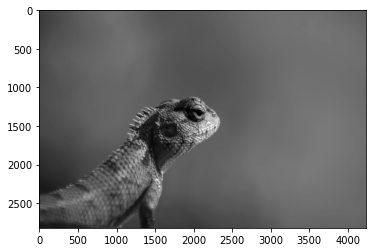
\includegraphics[width=0.9\columnwidth]{citra-gs.png}}
        \caption{Citra berwarna 8-bit)}
        \label{fig:8grayscale}
    \end{figure}

    \item \textbf{Citra 1-bit} \\
    Citra 1-bit ini biasa dikenal dengan citra biner. Citra ini hanya memiliki dua kemungkinan nilai pixel, yaitu 0 atau 1. Jenis citra ini biasa digunakan
    sebagai \emph{masking} dalam pengolahan citra. Citra pada figur \ref{fig:1binary} adalah hasil konversi pada citra figur \ref{fig:24original} menjadi citra biner.

    \begin{figure}[htbp]
        \centerline{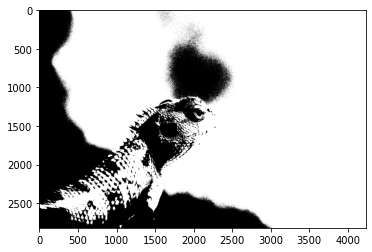
\includegraphics[width=0.9\columnwidth]{citra-bin.png}}
        \caption{Citra berwarna 1-bit}
        \label{fig:1binary}
    \end{figure}

\end{itemize}

\subsection{Keterbagian Bilangan Bulat}
Pembagian merupakan konsep penting yang menjadi dasar dari teori bilangan. Sebuah bilangan dapat membagi habis bilangan lain. Definisi dari habis dibagi dapat dilihat pada
definisi \ref{def:divided}.

\begin{definition} \label{def:divided}
    Misalkan $x$ dan $y$ adalah sebuah bilangan bulat. Dapat dikatakan $x$ habis membagi $y$ atau dinotasikan dengan
    $$ a | b $$
    jika dan hanya jika terdapat sebuah bilangan bulat $a$ yang memenuhi persamaan $ y = ax $
\end{definition}

Dalam berbagai bilangan bulat, terdapat satu kelompok bilangan bulat  yang sangat penting yaitu bilangan prima.
\begin{definition} \label{def:prime}
    Sebuah bilangan bulat $x$ dengan $x > 0$ dikatakan bilangan prima jika dan hanya jika bilangan tersebut hanyalah habis dibagi oleh $x$ dan 1.
\end{definition}

Terdapat teorema penting mengenai bilangan prima yang disebut dengan teorema fundramental aritmatik. \cite{b2}

\begin{theorem}[Teorema Fundramental Aritmatik]
    Setiap bilangan bulat positif yang lebih dari sama dengan 2 dapat dinyatakan sebagai perkalian yang setidaknya terdapat sebuah bilangan prima. 
\end{theorem}

Setiap bilangan prima yang dapat membagi sebuah bilangan bulat disebut dengan faktor prima.

\subsection{Aritmatika Modulo}
Dalam teori bilangan dikenal sebuah operasi yang disebut dengan operasi aritmatika modulo. Aritmatika modulo ini memainkan peran penting dalam Kriptografi untuk membantu
mengamankan data. Operator yang digunakan pada operasi modulo adalah $ \text{mod} $. Operasi ini didefinisikan pada definisi \ref{def:modulo}.

\begin{definition} \label{def:modulo}
    Misalkan $x$ dan $m$ adalah sebuah bilangan bulat dengan $ m > 0 $. Kesamaan $ x \mod{m} = r $ merupakan kesamaan semedikian sehingga $ x = ma + r $ dengan nilai $0 \le r < m$.
    Dengan kata lain, $r$ adalah sisa bagi dari pembagian $x$ dan $m$.
\end{definition}

Dalam aritmatika modulo, terkadang dua buah bilangan bisa saja memiliki hasil modulo yang sama. Kedua bilangan ini bisa disebut kongruen dalam suatu modulo. Kekongruenan ini dapat
didefinisikan sebagaimana definisi \ref{def:congruent}.

\begin{definition} \label{def:congruent}
    Misalkan terdapat tiga buah bilangan bulat $a$, $b$, dan $m$ dengan $m > 0$. Dapat dikatakan bahwa bilangan $a$ dan $b$ kongruen atau dengan notasi
    $$ a \equiv b \text{ } (\text{mod } m) $$
    jika dan hanya jika $a-b$ habis dibagi oleh $m$.
\end{definition}

\subsection{Pembagi Bersama Terbesar}
Dua buah bilangan bulat bisa saja habis dibagi dengan suatu bilangan bulat. Pembagi ini bisa saja lebih dari satu. Akan tetapi, terdapat sebuah bilangan pembagi dari kedua buah bilangan
bulat tersebut yang disebut dengan pembagi bersama terbesar (PBB) atau disebut dengan \emph{greatest common divisor} (GCD). 

\begin{definition} \label{def:gcd}
    Misalkan terdapat dua buah bilangan bulat $a$ dan $b$ dengan $a,b > 0$. Dikatakan $x$ merupakan $\gcd{(a,b)}$ jika dan hanya jika $x$ bilangan bulat terbesar yang memenuhi $x | a$ dan $x | b$.
\end{definition}

Terdapat sebuah istilah yang cukup penting, yaitu relatif prima. Dua buah bilangan bisa dikatakan relatif prima bila memenuhi definisi \ref{def:relativeprime}.

\begin{definition} \label{def:relativeprime}
    Misalkan terdapat dua buah bilangan bulat $a$ dan $b$ dengan $a,b > 0$. Dikatakan $a$ relatif prima dengan $b$ jika dan hanya jika $\gcd{(a,b)} = 1$.
\end{definition}

\subsection{Pembangkit Bilangan Acak}
Dalam dunia keinformatikaan, bilangan acak merupakan bilangan yang sangat dibutuhkan. Bilangan acak sangat diperlukan terutama dalam kriptografi. Terdapat berbagai jenis pembangkit bilangan acak,
salah satunya adalah \emph{Linear Congruential Generator} (LCG). Bilangan acak ini didefinisikan dalam relasi rekurens pada persamaan \ref{eq:lcg}.

\begin{equation} \label{eq:lcg}
    x_{i+1} = ax_{i}+b \text{ (mod }m\text{)}
\end{equation}

Untuk memulai LCG, diperlukan sebuah umpan yaitu $x_0$. Dengan umpan yang sama, dapat didapatkan sebuah nilai urutan yang sama. 
Parameter $a$, $b$ dan $m$ sangat menentukan periode dari LCG. Terdapat sebuah teorema
yang dapat membantu menentukan nilai $a$, $b$, dan $m$ agar memperoleh periode maksimum. \cite{a1}

\begin{theorem}[Teorema Hull–Dobell]
    Sebuah LCG yang didefinisikan pada definisi \ref{eq:lcg} dapat memiliki periode penuh, yaitu berperiode $m-1$ jika memenuhi syarat berikut:
    \begin{enumerate}
        \item $b$ relatif prima terhadap $m$,
        \item $a \equiv 1 \text{(mod }p\text{)}$ jika $p$ merupakan faktor prima dari $m$,
        \item $a \equiv 1 \text{(mod }4\text{)}$ jika $m$ adalah bilangan yang habis dibagi oleh 4.
    \end{enumerate}
\end{theorem}

\section{Pembahasan}

\begin{thebibliography}{00}
\bibitem{b1} Munir, Rinaldi. 2019. \emph{Kriptografi Edisi Kedua}. Bandung: Penerbit Informatika 
\bibitem{b2} Munir, RInaldi. 2020. \emph{Matematika Diskrit Revisi Ketujuh}. Bandung: Penerbit Informatika
\bibitem{b3} HIdayatullah, Priyanto. 2017. \emph{Pengolahan Citra Digital Teori dan Aplikasi Nyata}. Bandung: Penerbit Informatika.
\bibitem{a1} Hull, T. E. \& Dobell, A. R. 1962. Random Number Generators. SIAM Review, 4(3), 233. http://chagall.med.cornell.edu/BioinfoCourse/PDFs/Lecture4/random\_number\_generator.pdf. Diakses pada 14-12-2021.
\end{thebibliography}

\end{document}
